\documentclass[12pt,a4paper]{article}
\linespread{1.0}
% Language setting
% Replace `english' with e.g. `spanish' to change the document language
\usepackage[english]{babel}
\usepackage[colorlinks,linkcolor=blue]{hyperref}
% Set page size and margins
% Replace `letterpaper' with `a4paper' for UK/EU standard size
\usepackage[letterpaper,top=2cm,bottom=2cm,left=3cm,right=3cm,marginparwidth=1.75cm]{geometry}

\usepackage[T1]{fontenc}
\usepackage[utf8]{inputenc}
\usepackage{authblk}
% Useful packages
\usepackage{amsmath}
\usepackage{graphicx}
\usepackage[colorlinks, linkcolor = blue]{hyperref}
% \usepackage{indentfirst} 
\usepackage{float}
\setlength{\parindent}{2em}
\title{Insurance charge estimation based on regression analysis}

\author[2]{Hanzheng Qiu}
\author[2]{Likun Lin}
\author[2]{Tianxing Sun}
\author[1]{Xiaoyang Li}
\author[2]{Zhenda Shen}
\affil[1]{Department of Computer Science, City University of Hong Kong}
\affil[2]{Department of Mathematics, City University of Hong Kong}
\begin{document}
\maketitle


\begin{abstract}
A dataset from Kaggle is collected on the relationship between individual medical expenditure and several mutually independent factors. Based on this dataset, we analyzed the relationship between factors, such as age, BMI, and healthcare expenditures. We further developed a regression model based on simple linear regression approach. A simple linear regression is conducted on the nonsmoker category which achieves an accuracy of 0.9 on the test set to be in the prediction interval. The smoker category is separated into the high-charge group and low-charge group. Multiple linear regression is conducted on both groups. The $R^{2}$ scores are both over 0.9. Finally, it is concluded that the health expenditure of all populations is linearly related to age, and the effect of BMI on health expenditure varies with or without smoking.


\end{abstract}

\section{Motivation and Background}
Health and medical care are one of the most concerned topics in the modern society. Proper health care coverage can contribute to social stability, development and well being. For the authorities worldwide, within a limited budget, it is imperative for relevant departments to arrange medical insurance expenditures accurately and reasonably. Therefore, the analysis and management of public and personal health care expenditure is a crucial topic of administration. 

\section{Objectives}
The main objective of this experiment is to assess whether several given factors have a linear or other relationship with medical expenditure under our data set using statistical and linear regression approaches and, if exist, give a reasonable and predictive linear regression model.

\section{Data Collections and Data Prepossessing}
\subsection{Data Collection}
 The dataset is collected on Kaggle, where the dependent variable of this dataset is personal medical expenditure(represented as charges in the following reports) and the independent variables are six factors: age, sex, BMI, number of children, smoking or not, and residential area in the U.S. Among them,  ‘Smoking’, and ‘residential area’ are categorical variables, and 'no. of children' is considered as small discrete integer variables. As a consequence, 'age' and 'BMI' are considered useful for our analysis. These data are considered quite complete and clean at acquisition. 
 
\subsection{Data Prepossessing}
Firstly, It is observed that the data label of 'smoker' and 'non-smoker' led to a significant gap in the insurance charge, just as figure 1 and figure 2 show. 

\begin{figure}[H]
\centering
\begin{minipage}[t]{0.48\textwidth}
\centering
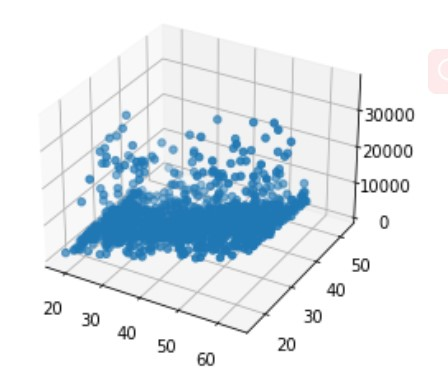
\includegraphics[width=6cm]{nonsmokeroverall.jpg}
\caption{Nonsmoker's condition}
\end{minipage}
\begin{minipage}[t]{0.48\textwidth}
\centering
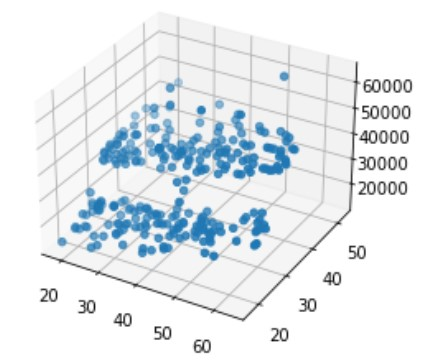
\includegraphics[width=6cm]{smokeroverall.jpg}
\caption{Smoker's condition}
\end{minipage}
\end{figure}

According to this observation, we are interested in whether it is reasonable to assume that the data in two labels are under different distributions. To examine this, we perform a hypothesis test on the mean of the two sets. Since both population mean and variance are unknown, we should perform the following test:
$$H_0: \mu_1=\mu_2,  H_1: \mu_1\ne \mu_2,$$
where $\bar{x_1}, s_2$ represents the sample(our data set) mean and variance charges for the smoker and $\bar{x_2}, s_2$ represents the sample mean and variance charges for the nonsmoker. Similarly, $\mu_1,\sigma_1$ represents the population means and variance charges for the smoker and $\mu_2,\sigma_2$ represents the sample mean and variance charges for the nonsmoker. 
Taking arbitrary sample from each of the two groups, the the random variable $\bar{X_1}-\bar{X_2}$ of the difference between their averages satisfies the following model
$$\frac{\left(\bar{X}_{1}-\bar{X}_{2}\right)-\left(\mu_{1}-\mu_{2}\right)}{\sqrt{\frac{S_{1}^{2}}{n_{1}}+\frac{S_{2}^{2}}{n_{2}}}} \stackrel{a}{\sim} t_{\nu}, \nu=\frac{\left(s_{1}^{2} / n_{1}+s_{2}^{2} / n_{2}\right)^{2}}{\frac{\left(s_{1}^{2} / n_{1}\right)^{2}}{n_{1}-1}+\frac{\left(s_{2}^{2} / n_{2}\right)^{2}}{n_{2}-1}}$$
From R code, the p-value $<2.2\times 10^{-16} $, which leads to the rejection of $H_0$ and we need to classify the data into smoker and nonsmoker for analysis. Separately 20 data from both categories are preserved to be test set and all remaining data form the training set.


\section{Clustering and Classification}
\subsection{Smokers' condition}

By observation of the BMI-charge(figure 3) and the age-charge(figure 4) figure, it is possible to separate the data from both graphs into two parts. 

\begin{figure}[H]
\centering
\begin{minipage}[t]{0.48\textwidth}
\centering
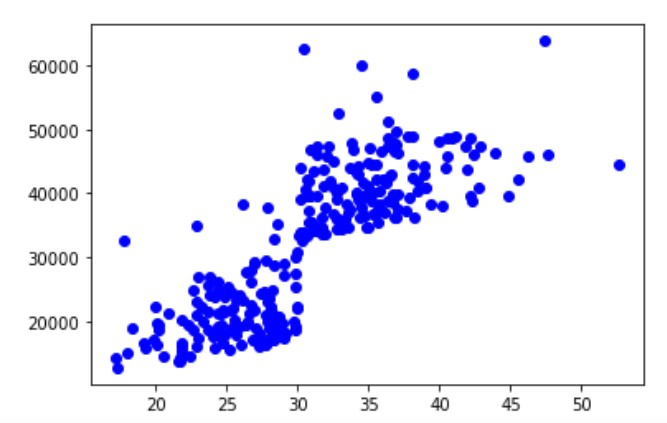
\includegraphics[width=6cm]{bmi-charge smoker.jpg}
\caption{BMI-charges figure}
\end{minipage}
\begin{minipage}[t]{0.48\textwidth}
\centering
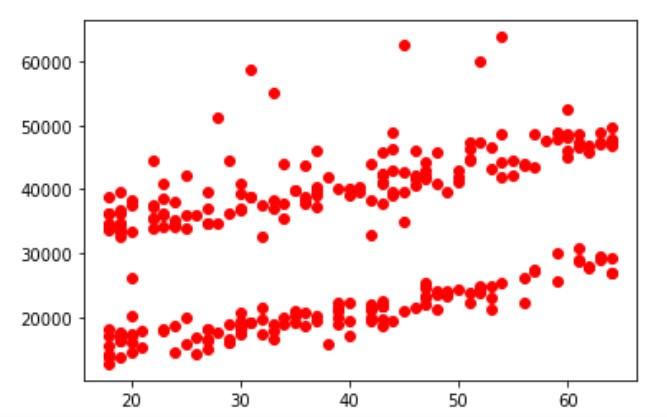
\includegraphics[width=6cm]{age-chargesmoker.jpg}
\caption{Age-charge figure}
\end{minipage}
\end{figure}


To do a more rigorous parting, Gaussian Mixture Model(GMM) is introduced to achieve this. For both graphs, the GMM model is set to do a two-cluster separation and achieves satisfying results as follows. As can be observed, even overlaying the two clustering together can almost separate the data points into two categories. One layer has obviously higher charges(over about 30,000) and higher BMI(over about 30) and the other's charges and BMI are lower.


\begin{figure}[H]
\centering
\begin{minipage}[t]{0.48\textwidth}
\centering
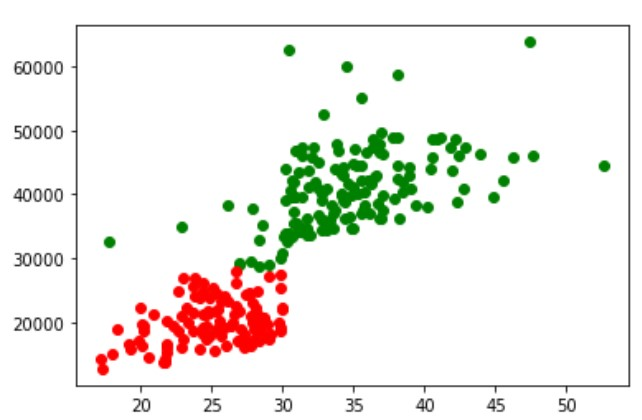
\includegraphics[width=6cm]{cluster result for bmi-charge.jpg}
\caption{clustering result for bmi-charge}
\end{minipage}
\begin{minipage}[t]{0.48\textwidth}
\centering
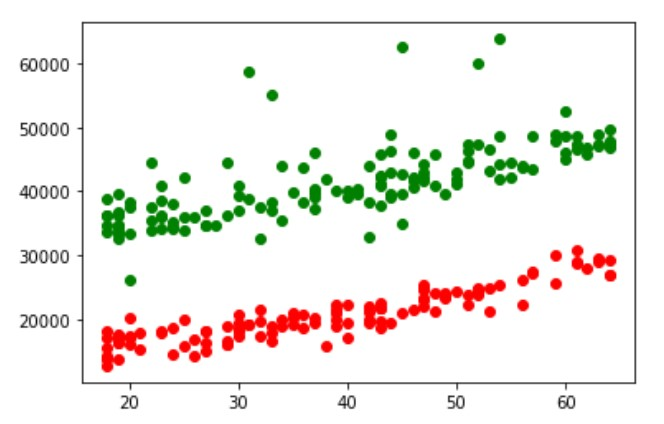
\includegraphics[width=6cm]{clustering result for age-charge.jpg}
\caption{clustering result for age-charge}
\end{minipage}
\end{figure}


According to the above analysis, the smoking population data can be divided into two categories: high charge and low charge. However, given that the goal is to predict costs based on BMI and age, a cost-independent classification method is needed. Therefore, the Support Vector Machine (SVM) was introduced to divide the data into two categories: high-charge and low-charge. According to the GMM labels, the results of age~bmi applied by the support vector machine are shown in Figure 7 and simple linear regression will be applied to these two distinct categories separately.

\begin{figure}[H]
\centering
\begin{minipage}[t]{0.48\textwidth}
\centering
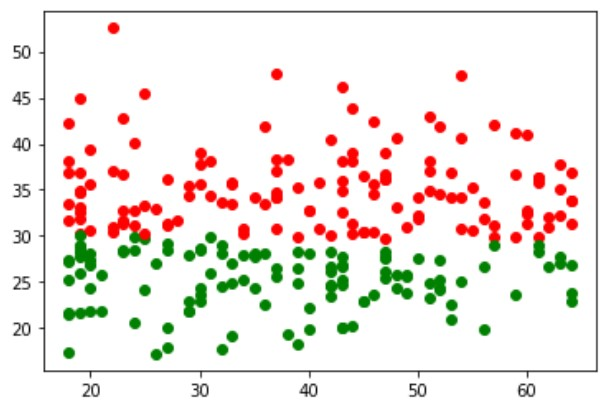
\includegraphics[width=6cm]{svm.jpg}
\caption{SVM Classification result}
\end{minipage}
\begin{minipage}[t]{0.48\textwidth}
\centering
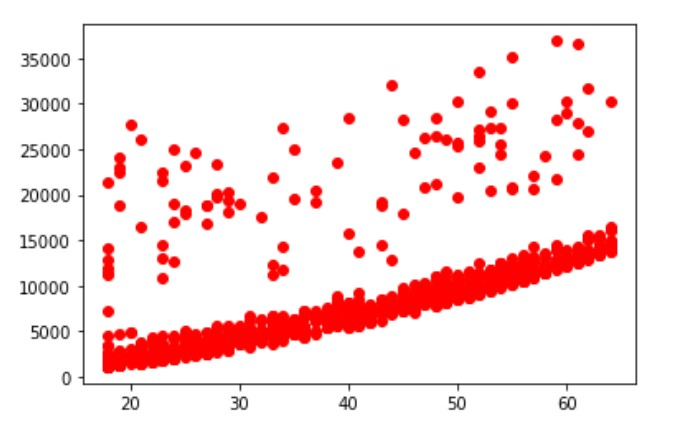
\includegraphics[width=6cm]{age-chargenonsmoker.jpg}
\caption{age-charge figure for non-smoker condition}
\end{minipage}
\end{figure}

\subsection{Non-smokers' condition}
By observation of the age-charges figure, The data are clustered densely in the low-charge area and scattered in the high-charge area. The GMM model is again used to cluster the data into two sets, whose result is in figure 9. The above clustering results projected onto age-bmi were shown in Figure 10, which is apparently terrible. Thus, the speculation is that we do not acquire enough data to perform a good classification among these data points. It may be caused by the lacking of customers with charges over 30000 but we do have not enough data to show. Consequently, what to be considered is merely cleaning the data by dropping out outliers and do not apply classification to the ‘non-smoker’ category afterward. 

\begin{figure}[H]
\centering
\begin{minipage}[t]{0.48\textwidth}
\centering
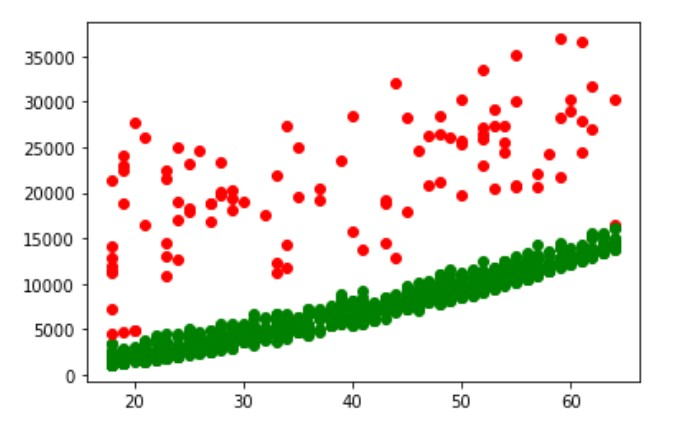
\includegraphics[width=6cm]{GMM RESULT with nonsmoker.jpg}
\caption{GMM result under nonsmoker condition}
\end{minipage}
\begin{minipage}[t]{0.48\textwidth}
\centering
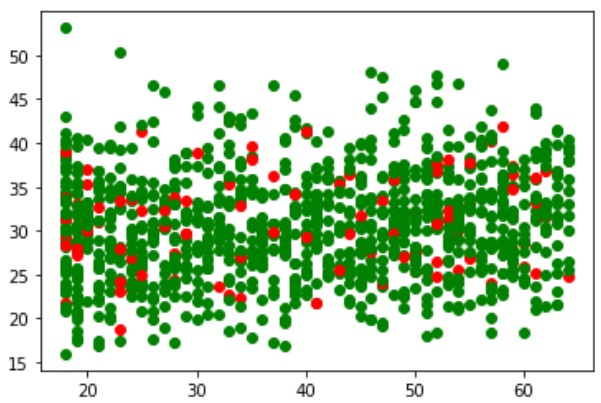
\includegraphics[width=6cm]{SVM2.jpg}
\caption{GMM cluster result on age bmi of non-smoker condition}
\end{minipage}
\end{figure}
In summary, currently, there are three categories, which are the nonsmoker category, the higher-charge smoker category, and the lower-charge smoker category.
\section{Linear Regression model}

\subsection{Simple Linear Regression with non-smoker category}
Firstly, the training set is cleaned by means of controlling the standardized residual between -2 and 2. 
Then, multiple linear regression is applied with the input features such as BMI and age, whose result is shown in figure 11. From the result, it is obvious that charges have almost no linear relationship with BMI, which shares the same conclusion as the ANOVA analysis in figure 12. 

\begin{figure}[H]
\centering
\begin{minipage}[t]{0.48\textwidth}
\centering
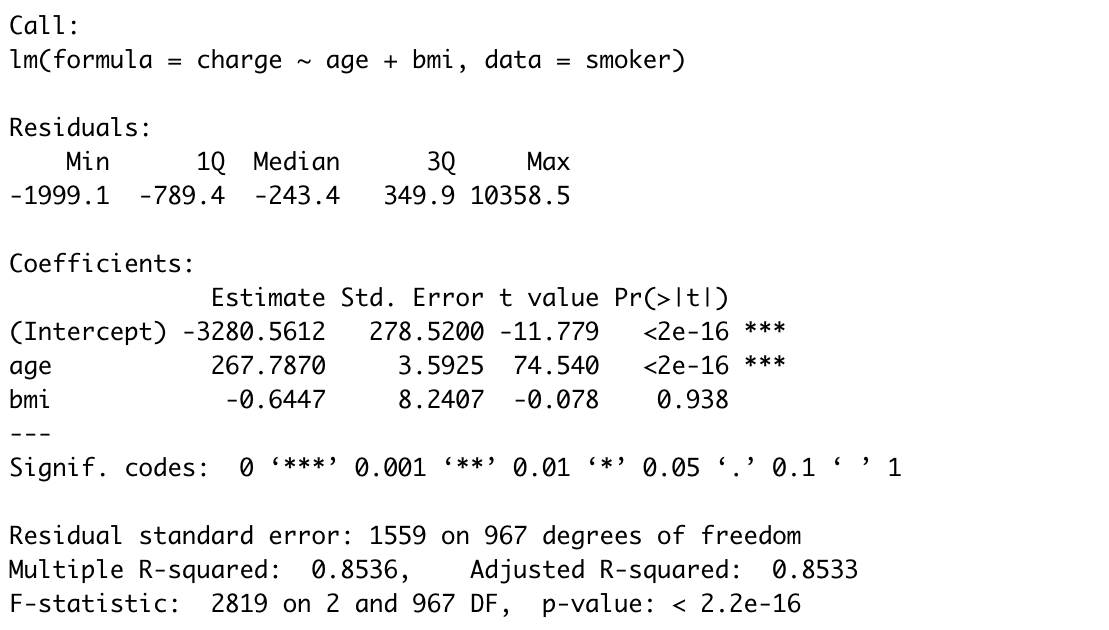
\includegraphics[width=6cm]{aftercleanlinear model.png}
\caption{Nonsmoker Multiple linear regression result}
\end{minipage}
\begin{minipage}[t]{0.48\textwidth}
\centering
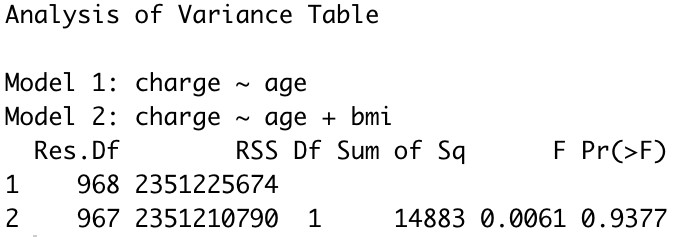
\includegraphics[width=6cm]{ANOVA.jpg}
\caption{Nonsmoker ANOVA analysis result}
\end{minipage}
\end{figure}

Consequently, Simple linear regression between age and charges is applied.
For input feature age (represented as X), the estimator for charges (represented as $\widehat{y}(x)$) can be calculated as:
$$\widehat{y}(x)=\widehat{\mu}_{Y \mid X=x}=\widehat{\beta}_{0}+\widehat{\beta}_{1} X $$,
The simple linear regression model from the R code is $Y = -3298.954 + 267.753x$, and $R^{2}$ is 0.8536, which is shown in figure 13.
Meanwhile, based on
$$\widehat{y}(x) \sim N\left(\mu_{Y \mid X=x}, \sigma^{2}\left(\frac{1}{n}+\frac{|x-\bar{x}|^{2}}{s_{x x}}\right)\right)$$
$$Y \mid(X=x)-\widehat{y}(x) \sim N\left(0, \sigma^{2}\left(1+\frac{1}{n}+\frac{|x-\bar{x}|^{2}}{s_{x x}}\right)\right)$$
With the unbiased estimator $s$ for $\sigma$, the  $0.95 $ confidence interval and the prediction interval are calculated and shown in figure 14.
The red dashed lines are the boundaries for the prediction interval and the grey band around the blue line is the confidence interval, which is very small.
The proportion for the test set to be in the prediction interval is 0.9, which is satisfying.

\begin{figure}[H]
\centering
\begin{minipage}[t]{0.48\textwidth}
\centering
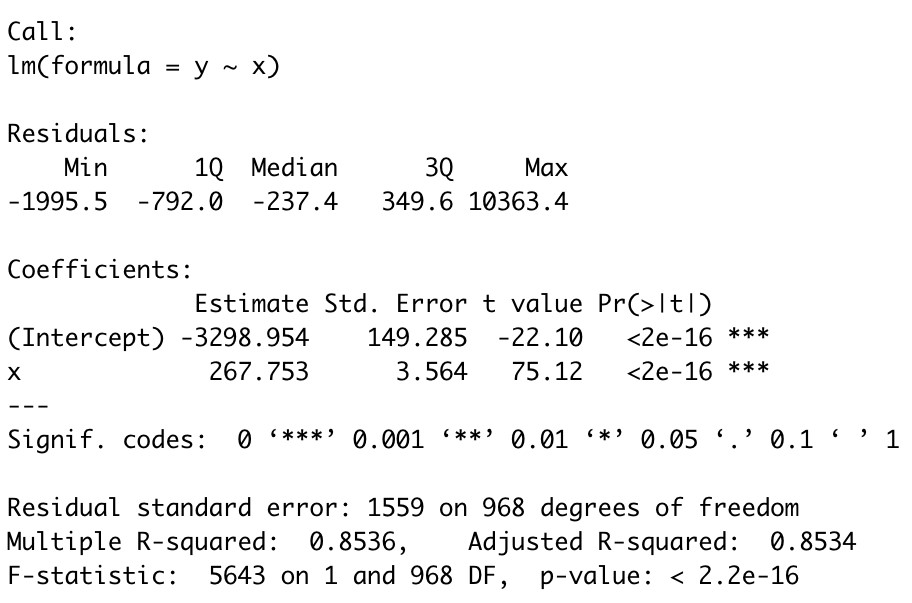
\includegraphics[width=6cm]{simple linear model.jpg}
\caption{Nonsmoker Multiple linear regression result}
\end{minipage}
\begin{minipage}[t]{0.48\textwidth}
\centering
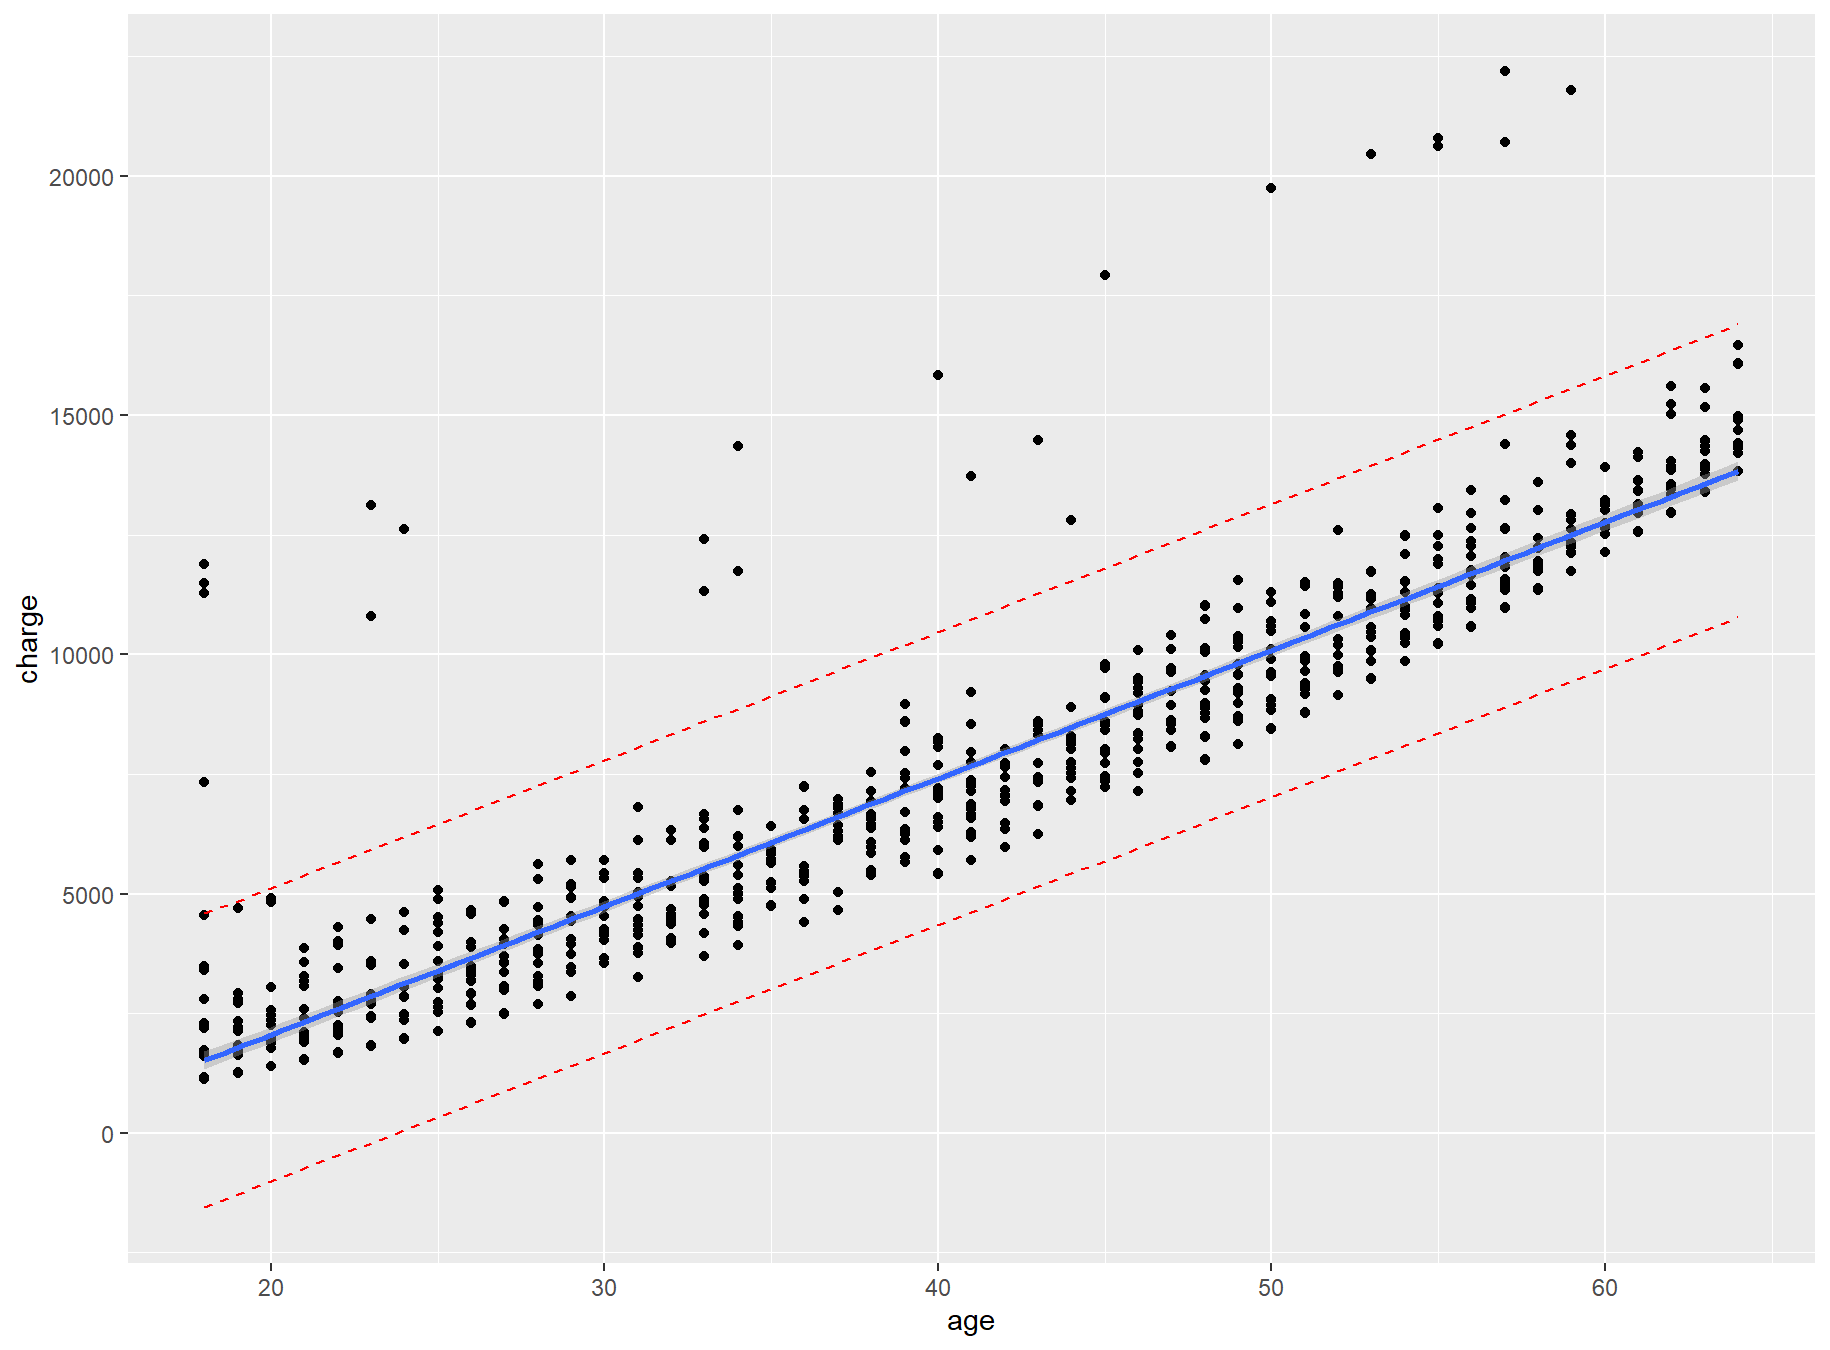
\includegraphics[width=6cm]{non_smoker.png}
\caption{Nonsmoker ANOVA analysis result}
\end{minipage}
\end{figure}

\subsection{Multiple Linear Regression with higher-charges smokers category }
Firstly, the training set is also cleaned by means of controlling the standardized residual between -2 and 2.
Then, multiple linear regression is applied with the input features such as BMI and age, whose result is shown in figure 15. From the result, it is obvious that charges have almost no linear relationship with BMI, which shares the same conclusion as the Added-variable plot in figure 16. 
\begin{figure}[H]
\centering
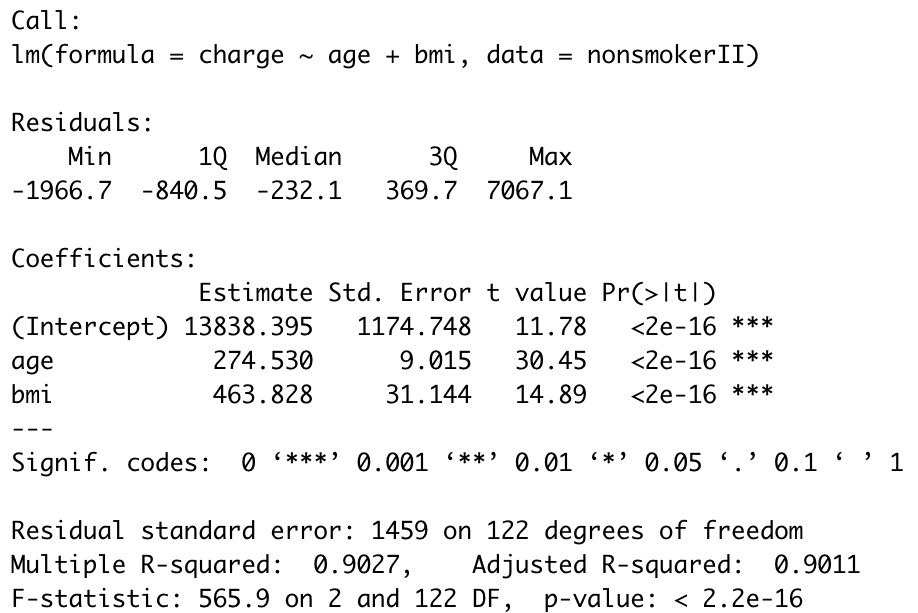
\includegraphics[width=0.48\textwidth]{mlm2.jpg}
\caption{Higher-charges smoker Multiple linear regression result}
\end{figure}

\begin{figure}[H]
\centering
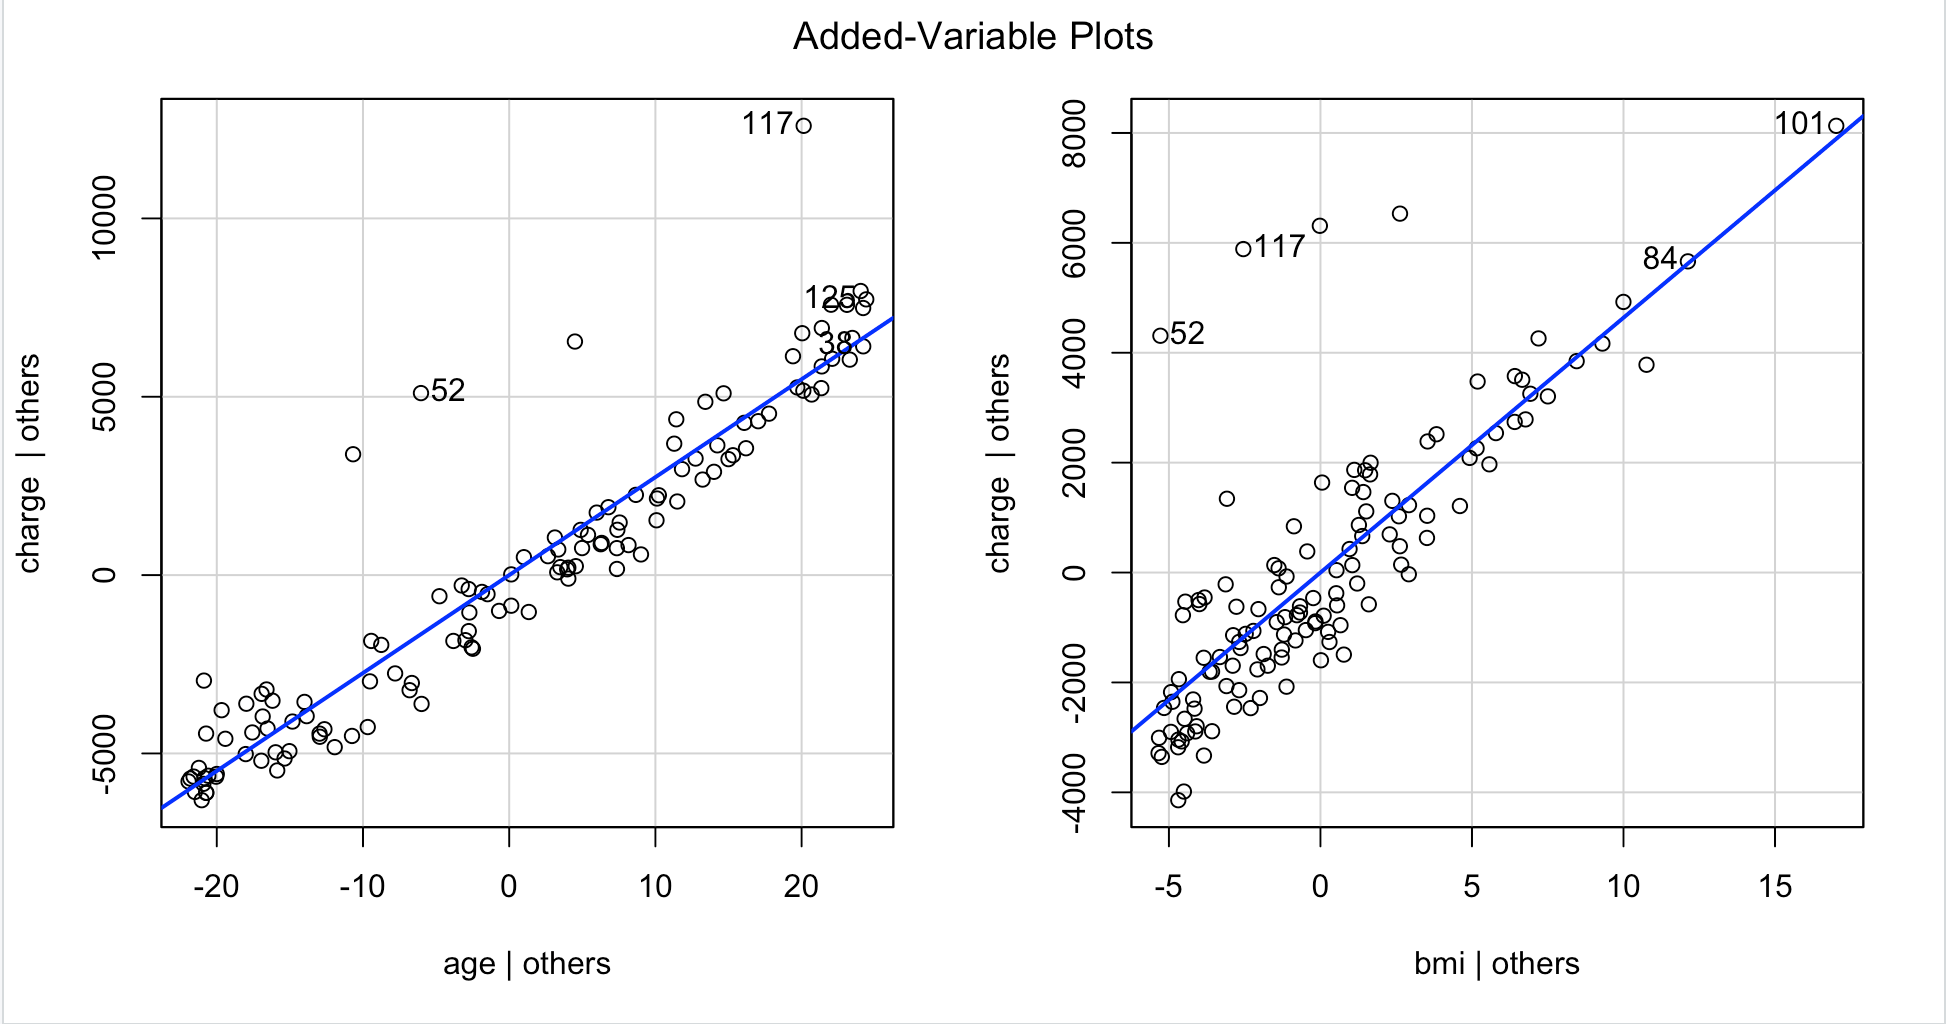
\includegraphics[width=1\textwidth]{avplot2.png}
\caption{Higher-charge smoker Added variable Plot result}
\end{figure}
For input feature age (represented as $X_1$), the estimator for charges (represented as $\widehat{y}(x)$) can be calculated as:
$$\widehat{y}(x)=\widehat{\mu}_{Y \mid X=\vec{x} }=\widehat{\beta}_{0}+\widehat{\beta}_{1} X_1+ \widehat{\beta}_{2} X_2$$,
The simple linear regression model from the R code is $Y = 13838.395 + 274.530 * X_1 + 463.828 * X_2$, and $R^{2}$ is  0.9027, which is shown in figure 15. The result is satisfying.
\subsection{Multiple Linear Regression with lower-charges smokers category}
Firstly, the training set is also cleaned by means of controlling the standardized residual between -2 and 2.
Then, multiple linear regression is applied with the input features such as BMI and age, whose result is shown in figure 17. From the result, it is obvious that charges have almost no linear relationship with BMI, which shares the same conclusion as the Added-variable plot in figure 18. 
\begin{figure}[H]
\centering
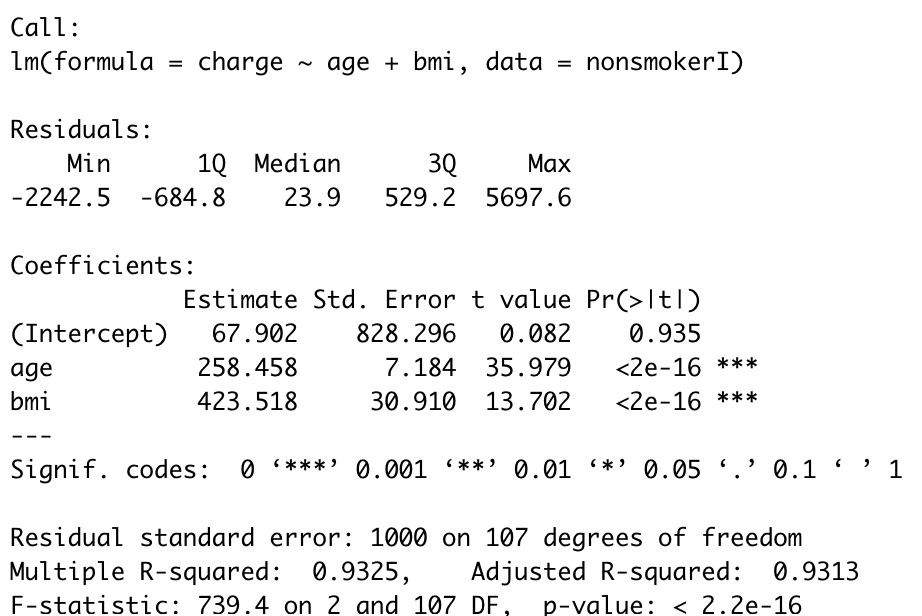
\includegraphics[width=0.48\textwidth]{mlm.jpg}
\caption{Lower-charges smoker Multiple linear regression result}
\end{figure}

\begin{figure}[H]
\centering
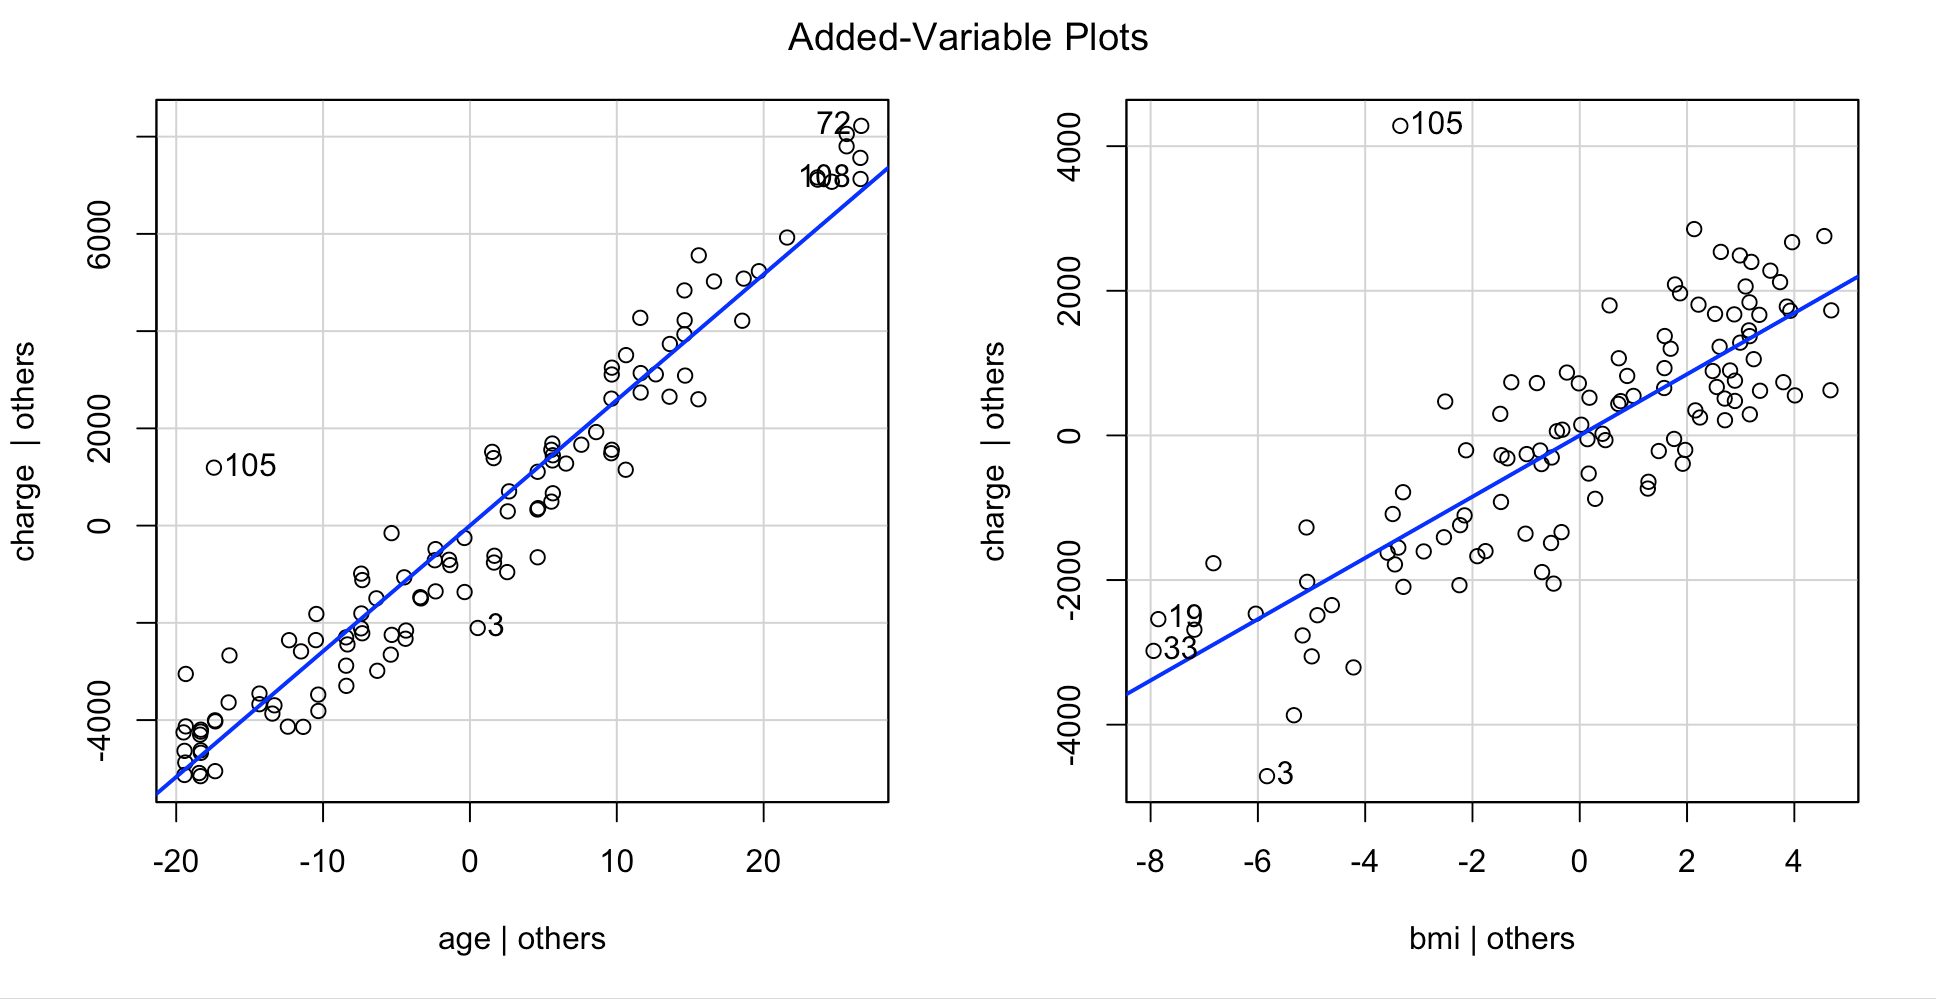
\includegraphics[width=1\textwidth]{avplot.png}
\caption{Lower-charge smoker Added variable Plot result}
\end{figure}

The simple linear regression model from the R code is $Y =  67.902 + 258.458 * X_1 +  423.518 * X_2$, and $R^{2}$ is 0.9325, giving a desirable result which is shown in figure 15.

\section{Summary of techniques used that is not taught in class}

Gaussian Mixture Model is used to cluster the data and the Support Vector Machine is used to classify the data.
\section{Conclusion}
This paper focused on the relationship between 'charge' and its independent variables 'smoker', 'BMI', and 'age'. Our discussion is based on the fact that different 'smoker' labels would lead to a significant difference in the value of charges. Further experiments proved that 'smokers' can be parted into different classes for their charges with respect to 'age' and 'BMI', while 'non-smokers' does not produce such a separating effect so only one class is adopted in the result. Generally speaking, the charge of the above three classes all possess a strong positive linear relationship with age. 
The result shows that our model may produce more errors when predicting the non-smoker category. It is suggested that relevant data, e.g. family status, is lacking in the present model, and thus further research can be conducted with aims of observing the relation between family and charge.


\section{Appendix}
Data source: \\
\url{https://www.kaggle.com/datasets/mirichoi0218/insurance}\\
.csv version: \\
 \url{https://drive.google.com/file/d/1_VQk7_KoigrBS3NEPzBX5rdbI6CE4w43/view?usp=sharing}\\
Our source code of R:\\ \url{https://github.com/AharenDaisuki/insurance_charges_estimation} \\
Python Prepossessing code: \\
 \url{https://drive.google.com/file/d/1VziKPOPhUNzKtoHm06vYHopCrpNNXNq-/view?usp=sharing}

\end{document}